% SPDX-License-Identifier: AGPL-3.0-or-later
% Commercial license available
% © Concepts 1996-2026 Miroslav Sotek. All rights reserved.
% © Code 2020-2026 Miroslav Sotek. All rights reserved.
% ORCID: 0009-0009-3560-0851
% Contact: www.anulum.li | protoscience@anulum.li
% scpn-quantum-control --- IQM Garnet preregistered campaigns manuscript

\pdfinfoomitdate=1
\pdfsuppressptexinfo=-1
\pdftrailerid{}

\documentclass[reprint,aps,physrev,superscriptaddress,floatfix,longbibliography]{revtex4-2}

\usepackage[T1]{fontenc}
\usepackage{amsmath,amssymb}
\usepackage{booktabs}
\usepackage{graphicx}
\usepackage{hyperref}
\usepackage{xcolor}
\usepackage{xurl}
\usepackage{enumitem}
\usepackage{microtype}
\setlist{nosep,leftmargin=*}
\setlength{\tabcolsep}{5pt}

\hypersetup{
    colorlinks=true,
    linkcolor=blue!60!black,
    citecolor=blue!60!black,
    urlcolor=blue!60!black,
    pdftitle={The calibration epoch as the unit of evidence: preregistered parity-leakage and layout-transfer experiments on IQM Garnet},
    pdfauthor={Miroslav \v{S}otek},
    pdfsubject={Preprint. Zenodo DOI 10.5281/zenodo.23298119. Hardware access: IQM Garnet through IQM Resonance.},
    pdfkeywords={IQM Garnet, superconducting qubits, parity-sector leakage, calibration epoch, preregistration, random-effects analysis, layout transfer, Kuramoto-XY},
    pdfcreator={},
    pdfproducer={},
}

\providecommand{\tightlist}{}
\newcommand{\paperdoi}{Zenodo DOI: \href{https://doi.org/10.5281/zenodo.23298119}{10.5281/zenodo.23298119}}

\begin{document}
\emergencystretch=3em
\raggedbottom

\title{The calibration epoch as the unit of evidence:\\ preregistered parity-leakage and layout-transfer experiments on IQM Garnet}

\author{Miroslav \v{S}otek}
\email{protoscience@anulum.li}
\affiliation{ANULUM, Marbach SG, Switzerland}
\affiliation{ORCID: 0009-0009-3560-0851}

\date{October 11, 2026\\ \mbox{\paperdoi}}

\begin{abstract}
We report five preregistered experiments on the IQM Garnet 20-qubit
square-lattice processor, each with its decision rule committed before any
hardware data existed and each reported regardless of outcome. First, the
even-over-odd parity-sector leakage asymmetry previously measured on IBM Heron
r2 replicates on Garnet at preregistered power (relative asymmetry +0.068,
one-sided \(p = 1.1\times 10^{-5}\)). Because the noiseless parity leakage of these
number-conserving XY-Trotter circuits is exactly zero, this is a statement
about device noise. Second, the asymmetry is not stable: over ten execution
windows it varies beyond shot noise at fixed depth (Cochran \(Q = 19.01\) on 9
degrees of freedom, \(p = 0.025\)), more strongly when windows are pooled by
provider calibration set (\(p = 0.0083\)), and an isolated sign reversal at depth
10 does not replicate. Third, a confirmatory campaign that takes the
calibration epoch as its independent unit --- twelve epochs, 688,128 shots ---
finds the asymmetry larger at depth 8 than at depth 12 (mean contrast +0.0173,
one-sided \(p = 0.026\)); the lower bound is +0.0030 and three of twelve epochs
have the opposite sign. Fourth, a calibration-aware layout optimiser developed
on heavy-hex devices fails its frozen transfer rule: it is better than
automatic placement at chain lengths 8 and 16 and worse at 12, and a powered
follow-up confirms the reversal. All preregistrations, calibration snapshots,
job identifiers, raw counts and analysis scripts are public.
\end{abstract}

\maketitle

\hypertarget{sec:1}{%
\section{Motivation and prior state}\label{sec:1}}

Two threads of our published programme meet on a square lattice.

First, the \textbf{layout thread}: our fidelity-aware placement stack --- a
community-detection analysis pass, a Kuramoto-XY-aware discrete layout cost
model, and a multi-restart discrete optimiser --- was built and benchmarked
entirely on IBM heavy-hex devices. Whether calibration-aware placement gains
survive a change of lattice topology is an open, publishable question in both
directions, and square-lattice Garnet is the natural second data point.

Second, the \textbf{parity thread}: on IBM Heron r2 (\texttt{ibm\_fez}, \texttt{ibm\_kingston}) we
measured a robust even-over-odd parity-sector leakage asymmetry in
number-conserving Kuramoto-XY~\cite{Kuramoto1975,Acebron2005} Trotter circuits (+10.8\,\% $\pm$ 1.1 pooled, Fisher
\(p \ll 10^{-16}\))~\cite{SotekSoftware2026}. An exact statevector baseline
subsequently proved the noiseless parity leakage of these circuits is exactly
zero at every depth (excitation-number conservation), reframing the result:
the asymmetry is a property of device noise, not of coherent dynamics, and
the live question became whether that noise structure is backend-universal~\cite{SotekDLA2026}. A 2026-05-13 Garnet pilot (six layouts,
12,288 shots) was too weak to answer: combined p between 0.05 and 0.57,
sign agreement 1/3 to 3/3 across layouts. Only layout {[}2, 7, 12, 13{]} agreed
with IBM in sign at all three depths --- which is why the present confirmatory
block pins that layout, discloses the selection, and treats the May data as
design input, never as evidence.

\hypertarget{sec:2}{%
\section{Methods common to both experiments}\label{sec:2}}

\textbf{Hardware access.} All quantum-hardware results in this work were obtained on IQM Garnet through \textbf{IQM Resonance}; we thank IQM for extended Resonance access. The two core experiments ran on 20 qubits of the square-lattice device on 2026-07-21 (calibration set \texttt{246a4930-54e3-4cd9-a2d1-fcc0919675f5}); explicitly identified follow-ups used fresh windows and their own recorded calibration sets. The window-variability campaign (Sec.~\ref{sec:6}) ran in ten windows between 2026-07-22 and 2026-09-04, and the depth-ordering confirmation (Sec.~\ref{sec:7}) in twelve calibration epochs between 2026-09-23 and 2026-10-06, each under its own recorded calibration set.

\textbf{Device and access.} IQM Garnet (20 qubits, square lattice)~\cite{Abdurakhimov2024} via IQM
Resonance, 2026-07-21, single calibration window. Live calibration was
snapshotted through the published quality-metrics endpoint before circuit
freezing (per-edge CZ gate fidelity; per-qubit readout error), committed as a
JSON artefact, and used both to drive the optimiser arm of Experiment 1 and to
verify layout availability for Experiment 2.

\textbf{Preregistration.} Both campaign documents were committed before execution
(\nolinkurl{docs/campaigns/iqm_layout_transfer_square_lattice_prereg_2026-07-21.md},
\nolinkurl{docs/campaigns/iqm_dla_backend_sensitivity_powered_prereg_2026-07-21.md}),
freezing hypotheses, endpoints, shot budgets, stop rules, and decision rules.
One pre-submission amendment was made to Experiment 1 (Sec.~\ref{sec:3-1}) before
any hardware data existed; the original text and the evidence that forced the
amendment are retained in the document.

\textbf{Readiness gates.} Neither experiment was submitted before passing: unit
tests to the repository standard (100\,\% line and branch coverage on the new
harness modules), a complete \texttt{IQMFakeGarnet} dry run of every circuit from
committed code, committed exact classical baselines, and --- for Experiment 1 ---
a transpiled two-qubit depth-parity gate across arms; for Experiment 2 --- a
transpiled depth envelope (May reference depth 159 + 25\,\%). A zero-spend
server-side \texttt{garnet:mock} submission validated the full submit--retrieve loop
before each first real block.

\textbf{Spend discipline.} Blocks were submitted incrementally, with dashboard
credit checks between blocks (the first block of each experiment carried a
preregistered abort threshold). The
entire dual campaign consumed roughly 13 of 30 monthly credits.

\hypertarget{sec:3}{%
\section{Experiment 1 --- layout-optimiser transfer to the square lattice}\label{sec:3}}

\hypertarget{sec:3-1}{%
\subsection{Design}\label{sec:3-1}}

Identical logical circuits per size: two-edge-colour width-2 XY-Trotter
chains (5 Trotter steps = 20 two-qubit layers, constant in n), initial state
at quarter filling (\texttt{1000} repeated), which fixes the conserved mean-Z
order-parameter proxy at exactly \(R = 0.5\) for every size and depth. The
endpoint, \(\mathrm{err}(\mathrm{arm}, n) = |R_{\mathrm{hw}} - 0.5|\), uses the absolute mean Z-magnetisation
proxy --- a sum of single-qubit marginals, so the two readout-calibration
circuits per size (all-zeros, all-ones over the union of measured qubits)
support an exact tensored per-qubit readout correction for this observable;
no full-matrix mitigation is claimed.

Three arms per size, identical circuits, different placements:

\begin{enumerate}
\def\labelenumi{\arabic{enumi}.}
\item
  \textbf{optimised} --- highest-fidelity connected chain region from the live
  calibration snapshot, order polished by the discrete Kuramoto layout
  optimiser under a deterministic, transpiler-free chain depth model;
\item
  \textbf{default} --- Qiskit~\cite{Qiskit2024} automatic placement (optimisation level 1, frozen
  transpiler seed);
\item
  \textbf{naive} --- calibration-blind topological baseline (Amendment 1): the
  lexicographically smallest connected chain on the coupling graph.
\end{enumerate}

\emph{Amendment 1 (pre-submission).} The originally preregistered naive arm ---
consecutive physical indices (0, \ldots, n$-$1) --- is not a connected path on Garnet;
the fake-backend readiness run showed routing SWAPs inflating its two-qubit
depth to 75/110/83 versus 40 for the other arms, violating the frozen
depth-parity validity gate at every size. The arm was redefined
(calibration-blind, topology-only) before any hardware data existed. After
amendment, all three arms transpile to identical two-qubit depth (40) at
every size, so fidelity differences are attributable to \emph{which} qubits and
edges are used, not to circuit volume.

Matrix: 3 sizes $\times$ 3 arms $\times$ 2,048 shots + 3 $\times$ 2 readout states $\times$ 1,024 shots
= 15 circuits, 24,576 + 6,144 shots. On the live calibration the three arms
separated onto genuinely different regions at \(n = 8\): optimised
(16, 11, 10, 15, 14, 13, 17, 18), default (1, 0, 3, 2, 7, 12, 13, 17), naive
(0, 1, 4, 3, 2, 7, 8, 9).

\textbf{Frozen primary rule.} \(\mathrm{err}(\mathrm{optimised}) < \mathrm{err}(\mathrm{default})\) at \textbf{all three}
sizes AND the bootstrap 90\,\% CI of the pooled error difference (10,000
shot-level multinomial resamples of every circuit including the readout
calibrations, seed 20260721) excludes zero. Secondary: \(\mathrm{err}(\mathrm{default})\) versus
\(\mathrm{err}(\mathrm{naive})\); two-qubit depth parity within 10\,\% as a validity gate.

\hypertarget{sec:3-2}{%
\subsection{Results}\label{sec:3-2}}

Table~\ref{tab:exp1} lists the readout-corrected order-parameter error versus the exact reference \(R = 0.5\)
(jobs \nolinkurl{019f8639-96be...}, \nolinkurl{019f8639-980e...}, \nolinkurl{019f8642-e162...},
\nolinkurl{019f8642-e326...}, \nolinkurl{019f8643-650c...}, \nolinkurl{019f8643-6712...}).

\begin{table}[tb]
\centering
\begin{tabular}{lllll}
\toprule
n & optimised & default & naive & optimised wins? \\
\midrule
8 & \textbf{0.1475} & 0.2533 & 0.2971 & yes \\
12 & 0.2088 & \textbf{0.1846} & 0.4138 & \textbf{no} \\
16 & \textbf{0.2924} & 0.3144 & 0.3378 & yes \\
\bottomrule
\end{tabular}
\caption{Experiment 1: readout-corrected order-parameter error against the exact reference $R=0.5$ for the three placements. Bold marks the smaller error of the optimised and default arms.}
\label{tab:exp1}
\end{table}

Pooled \(\mathrm{err}(\mathrm{default}) - \mathrm{err}(\mathrm{optimised})\) = \textbf{+0.0345}, bootstrap CI90
{[}+0.0260, +0.0431{]}. Pooled \(\mathrm{err}(\mathrm{naive}) - \mathrm{err}(\mathrm{default})\) = \textbf{+0.0989}, CI90
{[}+0.0898, +0.1079{]}. Depth parity held exactly (40/40/40 at every size). Figure~\ref{fig:layout} shows both runs.

\begin{figure*}[tb]
\centering
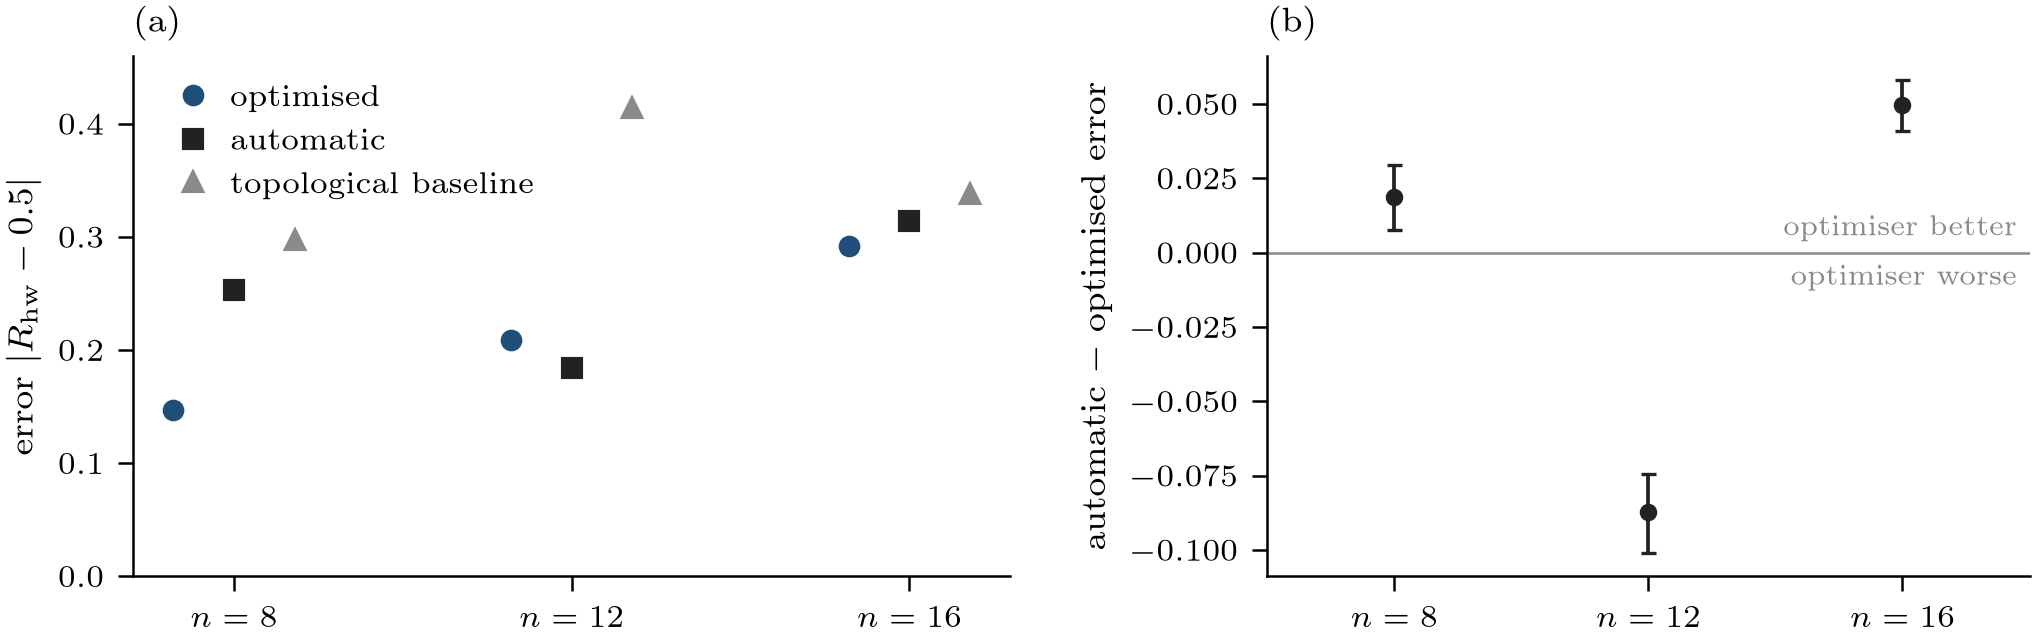
\includegraphics[width=0.98\linewidth]{figures/garnet_layout_transfer_by_chain_length}
\caption{Layout transfer on Garnet. (a) Readout-corrected order-parameter error of the three placements in the first experiment (2,048 shots per point). (b) Powered follow-up: corrected error of the automatic placement minus that of the optimised placement, with bootstrap 95\,\% intervals (8,192 shots per arm). The optimised placement is better at $n=8$ and $n=16$ and worse at $n=12$ in both runs.}
\label{fig:layout}
\end{figure*}

\hypertarget{sec:3-3}{%
\subsection{Interpretation (bounded, as preregistered)}\label{sec:3-3}}

\textbf{The frozen primary rule fails.} The all-sizes condition breaks at \(n = 12{,}\)
so no transfer claim is made --- even though the pooled interval excludes zero.
We report exactly the preregistered bounded conclusion:

\begin{itemize}
\item
  calibration-aware placement carries a real pooled advantage on this device
  and calibration window, but the advantage is \textbf{not uniform across sizes};
  the automatic transpiler matched or beat it at one of three sizes;
\item
  \textbf{placement itself matters strongly} on the square lattice: the
  calibration-blind topological baseline is worse than automatic placement at
  every size, by three times the optimiser's pooled margin.
\end{itemize}

A transfer claim therefore required a fresh design powered for per-size
conclusions and uniformity. That preregistered follow-up has now executed.

\hypertarget{sec:3-4}{%
\subsection{Powered per-size layout-transfer follow-up}\label{sec:3-4}}

The per-size layout-transfer study was frozen on 2026-07-22 before its
hardware data existed
(\nolinkurl{docs/campaigns/iqm_layout_transfer_per_size_prereg_2026-07-22.md}). It
repeated every arm four times at each size (8,192 main shots per arm/size),
added a fresh all-zero/all-one readout pair per size, and submitted the whole
42-circuit, 79,872-shot matrix in one pass on 2026-07-26 under calibration set
\texttt{c2097be4-1e23-49bc-adaa-8e8c01df6223}. Provider transpilation preserved an
identical two-qubit depth of 40 for every main circuit.

The frozen corrected \(\mathrm{default} - \mathrm{optimised}\) endpoint was significant at all
three sizes after Holm correction~\cite{Holm1979}, but not in one direction (Table~\ref{tab:persize}).

\begin{table*}[tb]
\centering
\begin{tabular}{lrlrl}
\toprule
n & default $-$ optimised & bootstrap CI95 & Holm p & direction \\
\midrule
8 & $+0.01868$ & {[}+0.00755, +0.02968{]} & 0.001200 & optimiser advantage \\
12 & \textbf{$-$0.08728} & {[}$-$0.10090, $-$0.07459{]} & 0.000600 & \textbf{optimiser disadvantage} \\
16 & $+0.04964$ & {[}+0.04109, +0.05823{]} & 0.000600 & optimiser advantage \\
\bottomrule
\end{tabular}
\caption{Powered per-size follow-up: corrected default-minus-optimised error with bootstrap 95\,\% intervals and Holm-adjusted $p$ values.}
\label{tab:persize}
\end{table*}

The powered design therefore confirms, rather than resolves away, the \(n = 12\)
reversal. Cochran's heterogeneity statistic~\cite{Cochran1954} rejects a common effect across
sizes (\(Q = 292.43\) on 2 df, \(p = 3.16\times 10^{-64}\)). Raw-count sensitivity preserves
all three directions. The pooled difference is slightly negative ($-$0.00632,
CI90 {[}$-$0.01187, $-$0.00099{]}) because the \(n = 12\) disadvantage dominates; it must
not be used to erase the per-size result. This is a size-dependent layout
effect in one Garnet calibration window, not a quantum-advantage,
backend-universal, or calibration-aware-superiority claim.

\hypertarget{sec:4}{%
\section{Experiment 2 --- parity-sector noise asymmetry at preregistered power}\label{sec:4}}

\hypertarget{sec:4-1}{%
\subsection{Design}\label{sec:4-1}}

Committed May-campaign builders, bit-identical circuits: \(n = 4\) XY-Trotter
chains, states \texttt{0011} (even sector) and \texttt{0001} (odd sector), depths 4, 6, 10,
four repetitions per state/depth at 1,024 shots (calibration-drift
resolution), plus one four-state readout block (\texttt{0011}, \texttt{0001}, \texttt{0000},
\texttt{1111} at 2,048 shots) --- 28 circuits, 32,768 shots, all on the pinned layout
{[}2, 7, 12, 13{]} (fallback {[}9, 4, 3, 8{]} was not needed; all three layout edges
were calibrated, CZ fidelities 0.982--0.990). Transpiled depths at submit
time: 69 / 99 / 159 for depths 4 / 6 / 10 --- the deepest exactly reproducing
the May envelope reference of 159, within the frozen +25\,\% bound of 198.

\textbf{Frozen primary.} Pooled across depths and repetitions (12,288 shots per
arm), one-sided two-proportion z-test of \(\mathrm{leak}_{\mathrm{even}} > \mathrm{leak}_{\mathrm{odd}}\) at \(\alpha = 0.05\);
committed power analysis: 90\,\% power at +0.044 relative asymmetry (the
weakest IBM per-depth reference). Secondary: per-depth Wilson intervals and
one-sided tests, per-repetition drift table, sign agreement with the IBM
direction. Claim boundary: with noiseless leakage exactly zero, every
statement is about device noise; no coherent-dynamics claim is available.

\hypertarget{sec:4-2}{%
\subsection{Results}\label{sec:4-2}}

Jobs \nolinkurl{019f866c-9c99...}, \nolinkurl{019f866c-9f20...}, \nolinkurl{019f8677-33b7...}, \nolinkurl{019f8677-7a0b...},
\nolinkurl{019f8677-ca9a...}

\textbf{Primary: H0 rejected.} Pooled \(\mathrm{leak}_{\mathrm{even}}\) = 0.4194 \textgreater{} \(\mathrm{leak}_{\mathrm{odd}}\) = 0.3928;
relative asymmetry \textbf{+0.0677}; \(z = 4.247\); one-sided \textbf{\(p = 1.1\times 10^{-5}\)}.
Garnet shows a positive even-over-odd parity-sector leakage asymmetry in the
IBM direction at preregistered power.

\textbf{Secondary depth profile.} Disclosed, not preregistered as an endpoint (Table~\ref{tab:exp2depth}).

\begin{table*}[tb]
\centering
\begin{tabular}{llllll}
\toprule
depth & \(\mathrm{leak}_{\mathrm{even}}\) & \(\mathrm{leak}_{\mathrm{odd}}\) & relative asymmetry & one-sided p & sign = IBM? \\
\midrule
4 & 0.3811 & 0.3098 & \textbf{+0.230} & $5.8\times 10^{-12}$ & yes \\
6 & 0.4197 & 0.3875 & \textbf{+0.083} & $1.5\times 10^{-3}$ & yes \\
10 & 0.4575 & 0.4812 & \textbf{$-$0.049} & 0.98 & \textbf{no} \\
\bottomrule
\end{tabular}
\caption{Experiment 2: secondary depth profile of the parity-sector leakage. Disclosed, not a preregistered endpoint.}
\label{tab:exp2depth}
\end{table*}

\hypertarget{sec:4-3}{%
\subsection{Interpretation}\label{sec:4-3}}

The pooled IBM-direction asymmetry replicating on a second superconducting
architecture --- square-lattice Garnet after heavy-hex Heron r2 --- is evidence
against the asymmetry being an artefact of one device family. To be precise
about what the two devices share and what they do not: \textbf{shared} is the
pooled even-over-odd sign of the parity-sector leakage asymmetry at
statistical power; \textbf{divergent} is the depth dependence (flat on IBM,
decaying and sign-reversing on Garnet), which may well reflect a different
underlying mechanism. ``Replication'' here therefore binds only to the pooled
directional effect, not to a claim that the two devices exhibit the same
noise structure.

\begin{figure*}[tb]
\centering
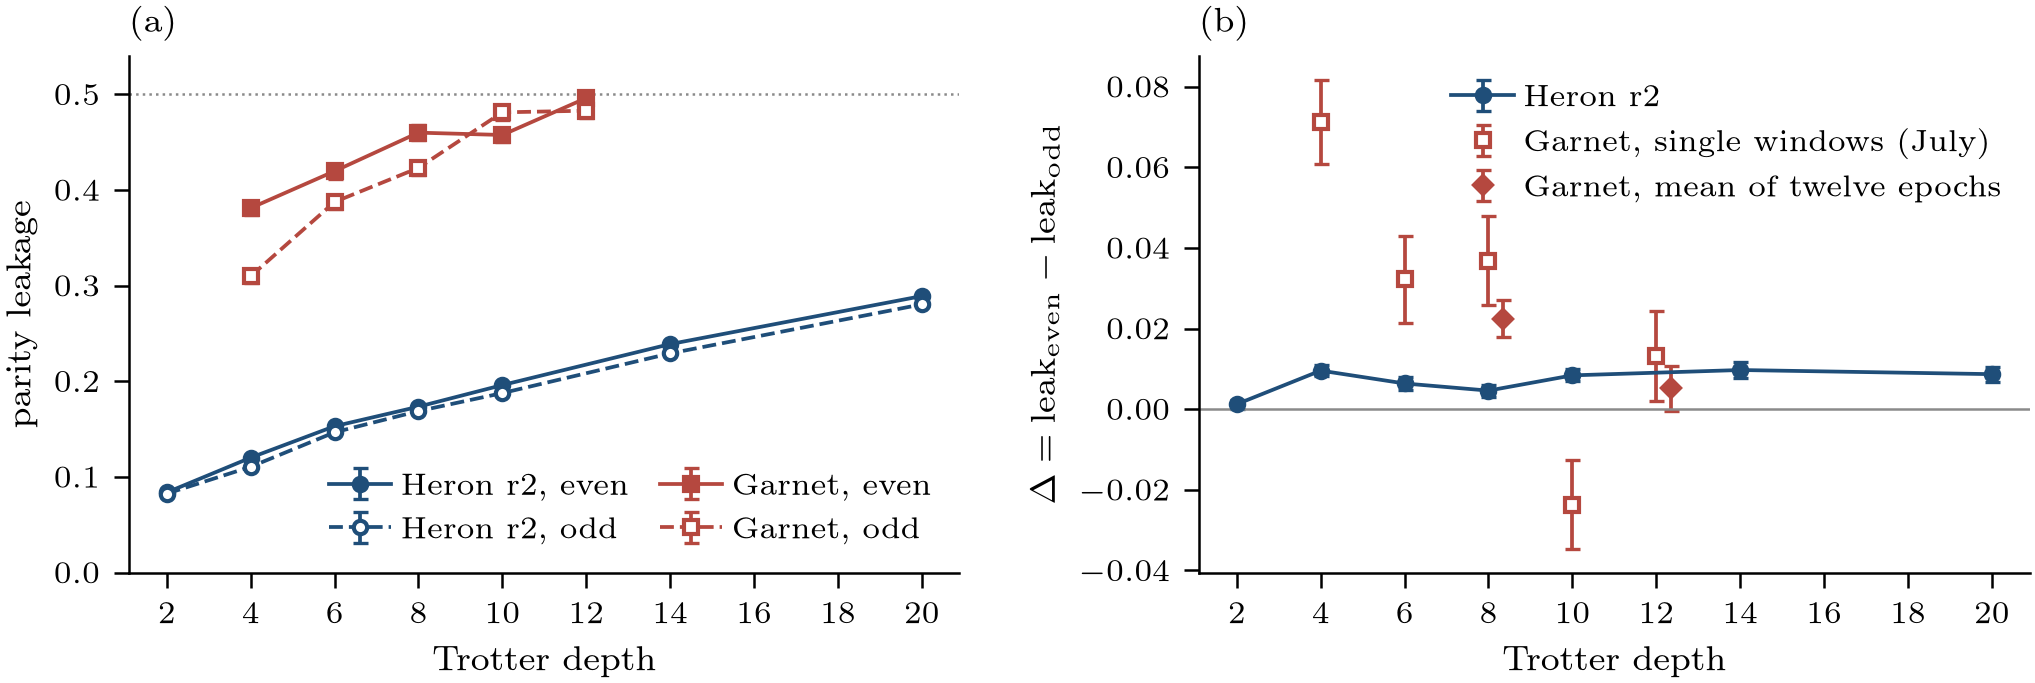
\includegraphics[width=0.98\linewidth]{figures/heron_garnet_parity_leakage_by_depth}
\caption{Parity-sector leakage of the four-qubit XY-Trotter circuits on IBM Heron r2 (\texttt{ibm\_kingston}, Phase 2 reference) and on IQM Garnet. (a) Leakage of the even and odd sectors; the dotted line is the fully mixed value. (b) Even-minus-odd difference. Open squares: single Garnet windows of July 2026 (4,096 shots per arm, binomial standard errors). Diamonds: random-effects means over the twelve calibration epochs of Sec.~\ref{sec:7}, offset horizontally for legibility. Heron r2 error bars are standard errors over 30 repetitions. Descriptive comparison, not a preregistered endpoint.}
\label{fig:devices}
\end{figure*}

Put side by side (Fig.~\ref{fig:devices}), the two devices differ first in scale. On \texttt{ibm\_kingston}
(the Phase 2 reference: 30 repetitions per sector and depth) the parity
leakage of this circuit family rises from 0.08 at depth 2 to 0.28--0.29 at
depth 20, and the even-minus-odd difference stays between +0.005 and +0.010
from depth 4 to depth 20. On Garnet the leakage is already 0.31--0.38 at depth
4 and reaches 0.48--0.50, the value of a fully mixed parity, at depth 12; the
difference is +0.071 at depth 4 in the July window and shrinks as the leakage
saturates. Garnet thus reaches within twelve Trotter steps a regime that Heron
r2 has not reached at twenty. The devices share the sign of the asymmetry and
differ in its size and in its dependence on depth. The comparison is
descriptive: different days, different numbers of repetitions, and not a
preregistered endpoint.

The initial secondary profile was qualitatively different from IBM's:
IBM's reference asymmetry was approximately flat in depth ($\approx$ +0.044 to
+0.087), while the first Garnet window fell from +0.230 at depth 4 to
$-$0.049 at depth 10. That isolated negative point initially motivated a
zero-crossing hypothesis, but it was not a preregistered endpoint. The
preregistered follow-ups in Sec.~\ref{sec:5} do not support that hypothesis: the
depth-8 versus depth-12 ordering is a bounded null (\(p = 0.064\)), a powered
fresh-window depth-10 retest is positive, and the two depth-10 windows differ
significantly (\(p \approx 0.006\)). The surviving bounded interpretation is therefore
window-to-window variability of device-noise asymmetry, not a depth-localised
zero crossing. No zero-crossing or equilibration-mechanism claim is made.

\hypertarget{sec:5}{%
\section{Preregistered depth-profile follow-up}\label{sec:5}}

A depth-profile campaign (depths 8 and 12, same layout, states, builders,
and shot discipline; 20 circuits, 24,576 shots) was preregistered separately
(\nolinkurl{docs/campaigns/iqm_dla_depth_profile_prereg_2026-07-22.md}) --- frozen
before any of its data existed --- and executed on 2026-07-22 under the same
calibration set as Experiment 2 (jobs \nolinkurl{019f8772-6338...}, \nolinkurl{019f8772-665d...},
\nolinkurl{019f87eb-30b1...}, \nolinkurl{019f87eb-f2f8...}, \nolinkurl{019f87ec-81b0...}).

\textbf{Its frozen primary (decay ordering) fails to reject the null:}
$\Delta_{8}$ = +0.0369 exceeds $\Delta_{12}$ = +0.0132 in the hypothesised direction, but the
one-sided test gives \(z = 1.52\), \(p = 0.064\) \textgreater{} 0.05, so the decay ordering is
not established at the committed power and we report the bounded null with
the same prominence as any positive result.

Table~\ref{tab:joint} gives the secondary, descriptive structure across the joint profile (depths 4/6/10
from Experiment 2's execution window, 8/12 from this one --- a cross-window
comparison frozen into the preregistration, mitigated by the shared calibration set).

\begin{table}[tb]
\centering
\begin{tabular}{llll}
\toprule
depth & relative asymmetry & mean total leakage & sign \\
\midrule
4 & $+0.230$ & 0.345 & \(+\) \\
6 & $+0.083$ & 0.404 & \(+\) \\
8 & $+0.087$ & 0.442 & \(+\) \\
10 & $-0.049$ & 0.469 & \(-\) \\
12 & $+0.027$ & 0.489 & \(+\) \\
\bottomrule
\end{tabular}
\caption{Joint depth profile: depths 4, 6 and 10 from the execution window of Experiment 2, depths 8 and 12 from the depth-profile follow-up under the same calibration set.}
\label{tab:joint}
\end{table}

Two hypothesis-generating observations arose: the mean total leakage rises
monotonically toward 0.5, consistent with sector equilibration compressing
the asymmetry at depth; and the sign pattern (+, +, +, $-$, +) places the
depth-10 negative between positive neighbours, suggesting a window
fluctuation rather than a systematic zero crossing.

\textbf{A third preregistered campaign tested the second reading directly}
(\nolinkurl{docs/campaigns/iqm_dla_d10_retest_prereg_2026-07-22.md}, frozen before
its data; 8,192 shots per arm --- 90\,\% power at the observed $-$0.0237 effect,
which the depth-profile arms could not resolve; jobs \nolinkurl{019f8809-42d7...},
\nolinkurl{019f8809-448d...}). \textbf{The depth-10 negative sign does not replicate:} in
the fresh window the depth-10 asymmetry is positive (\(\mathrm{leak}_{\mathrm{even}}\) 0.4611 \textgreater{}
\(\mathrm{leak}_{\mathrm{odd}}\) 0.4478; +0.030 relative), the one-sided test for the negative
sign gives \(p = 0.956\), and the preregistered cross-window secondary finds
the two windows' depth-10 asymmetries genuinely differ (\(z = 2.74\),
two-sided \(p \approx 0.006\)). Per the frozen wording this strengthens --- without
proving --- the window-fluctuation reading; with the fresh-window point
positive, every depth in the joint profile carries a positive sign, and
the surviving open question is the size of the window-to-window
variability of the asymmetry at fixed depth, not a zero crossing.

\hypertarget{sec:6}{%
\section{Window-to-window variability of the asymmetry}\label{sec:6}}

Sec.~\ref{sec:5} left one question: how large is the window-to-window variability of
the parity-sector asymmetry at a fixed depth. A fourth campaign was
preregistered to measure it directly
(\nolinkurl{docs/campaigns/iqm_dla_window_variability_prereg_2026-07-22.md}). One
nominal window is a complete 36-circuit execution on the pinned layout {[}2, 7,
12, 13{]} at depths 4, 8, 10 and 12, submitted as one main job and one readout
job, with 4,096 shots per state and depth; the window is the unit of custody
and of the frozen analysis. Ten windows were executed between 2026-07-22 and
2026-09-04.

\textbf{Frozen primary (depth 10, window level).} The even-minus-odd leakage
difference is heterogeneous across the ten windows beyond shot noise: Cochran
\(Q = 19.01\) on 9 degrees of freedom, \(p = 0.025\), with a between-window standard
deviation \(\tau = 0.0115\) against a mean shot-noise standard error of 0.0109 and a
weighted mean difference of +0.0179. The preregistered rule ``drift exceeds shot noise'' is met (Fig.~\ref{fig:windows}).

\begin{figure*}[tb]
\centering
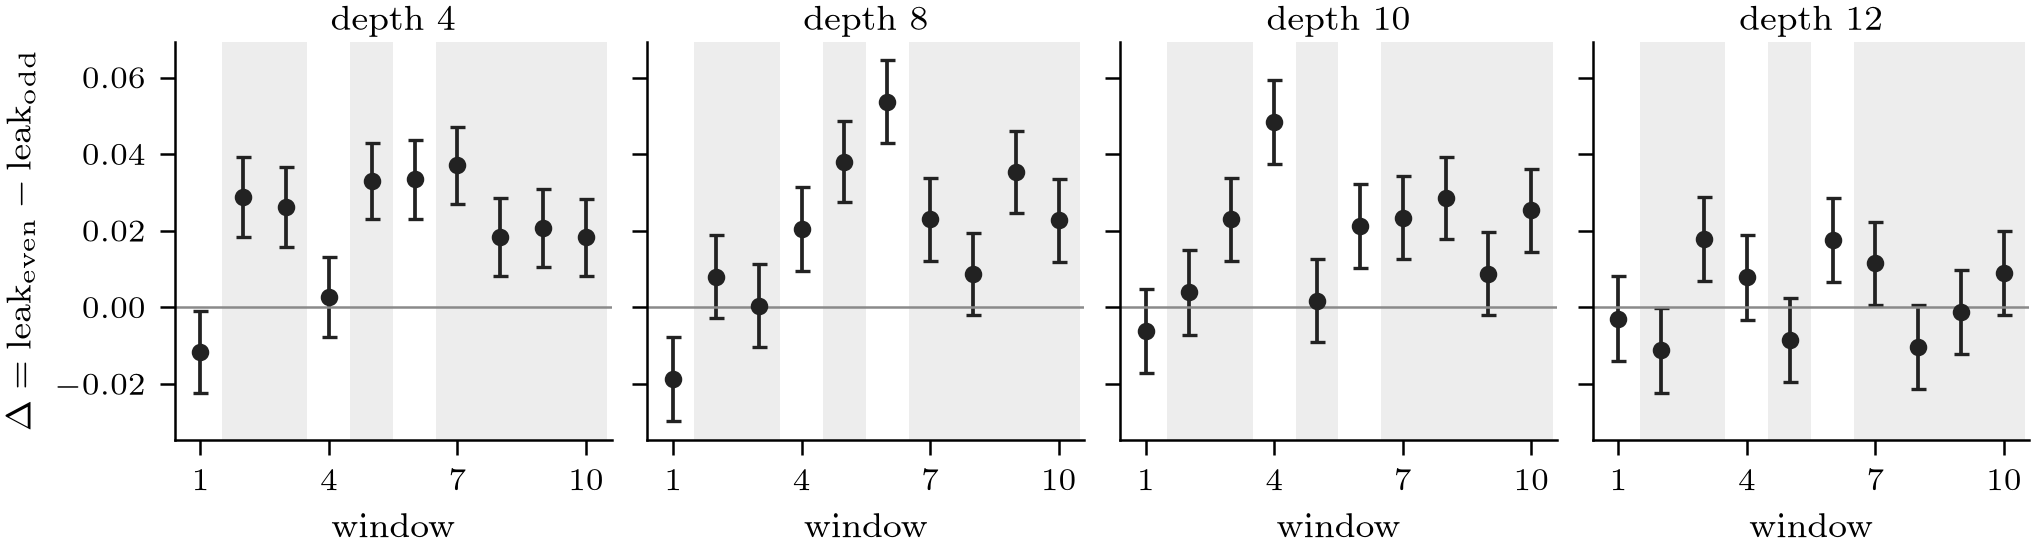
\includegraphics[width=0.98\linewidth]{figures/garnet_parity_asymmetry_ten_windows}
\caption{Even-minus-odd leakage difference on Garnet in the ten execution windows of the window-variability campaign, by depth. Error bars are binomial shot-noise standard errors (4,096 shots per arm). Shading alternates with the provider calibration set: windows inside one band were taken under the same calibration set and are technical replicates.}
\label{fig:windows}
\end{figure*}

\textbf{Secondary, by depth (Holm-adjusted).} Homogeneity is rejected at depth 8
(adjusted \(p = 4.4\times 10^{-4}\)) and not at depth 4 (0.053) or depth 12 (0.40). The
between-window $\tau$ is 0.0107, 0.0176, 0.0115 and 0.0022 at depths 4, 8, 10 and
12. The depth-4 difference is positive in nine of ten windows (Clopper--Pearson~\cite{ClopperPearson1934} 95\,\% interval 0.55 to 1.00).

\textbf{Calibration epochs (amendment, sensitivity analysis).} While the campaign
ran we found that several nominal windows carried the same provider
calibration set: windows 2--3 and windows 7--10. Windows under one calibration
set are technical replicates, not independent observations. An amendment
(\nolinkurl{docs/campaigns/iqm_dla_window_variability_epoch_amendment_2026-09-04.md}),
committed before windows 8 to 10 were counted for inference, adds an epoch-pooled analysis and requires both results to be reported together. Pooled to
six calibration epochs, the depth-10 heterogeneity is stronger, not weaker: Q
= 15.55 on 5 degrees of freedom, \(p = 0.0083\), \(\tau = 0.0129\) against a shot-noise
standard error of 0.0085. Homogeneity is rejected at depth 4 (adjusted \(p = 0.012\)) and depth 8 ($5.6\times 10^{-5}$), not at depth 12 (0.64; $\tau$ estimated at zero).

\textbf{What this establishes.} On this device and layout the parity-sector
asymmetry at depths 4, 8 and 10 varies between calibration epochs by an amount
comparable to or larger than the shot noise of a 4,096-shot arm. Adding shots
inside one calibration window therefore narrows the wrong interval: the
reported uncertainty of a single-window asymmetry understates how far the next
window will be. This is why the depth-ordering question of Sec.~\ref{sec:5} (one-sided \(p = 0.064\) inside one calibration set) could not be settled by more
shots, and it fixes the design of the confirmatory campaign that follows: the
calibration epoch is the independent unit.

\textbf{Boundary.} A changed calibration-set identifier marks an operational epoch;
it does not prove physical independence, and slow drift can cross calibration
boundaries. No cause of the variability is claimed; the calibration covariates
were preregistered as descriptive only.

\hypertarget{sec:7}{%
\section{Depth-ordering confirmation across calibration epochs}\label{sec:7}}

\textbf{Design.} Frozen before any of its data existed
(\nolinkurl{docs/campaigns/iqm_dla_depth_profile_powered_epoch_prereg_2026-09-04.md}).
The six calibration
epochs of Sec.~\ref{sec:6} gave the depth contrast C = (\(\mathrm{leak}_{\mathrm{even},8}\) $-$ \(\mathrm{leak}_{\mathrm{odd},8}\)) $-$
(\(\mathrm{leak}_{\mathrm{even},12}\) $-$ \(\mathrm{leak}_{\mathrm{odd},12}\)) a mean of 0.0164 and a between-epoch $\tau$ of 0.0150.
Those values were used to choose the sample size and for nothing else: their
counts and their six calibration sets are excluded from the confirmatory
endpoint. The campaign consists of twelve distinct, previously unused
calibration epochs. Each epoch runs the complete matrix in one pass: twelve
repetitions of each of the four state-by-depth cells at 1,024 shots (12,288
shots per cell), plus four readout states at 2,048 shots --- 48 main circuits in
one provider job and 4 readout circuits in a second, 57,344 shots per epoch
and 688,128 in total. An epoch is admitted only if its calibration set differs
from all earlier ones and from the six design epochs, every earlier epoch has
a complete paired calibration and count record, and the three edges of the
layout exist in the snapshot. No circuit, layout, depth, repetition or shot
count may change in response to a result; there is no optional stopping and no
replacement of an admitted epoch.

\textbf{Analysis (frozen).} A DerSimonian--Laird~\cite{DerSimonianLaird1986} random-effects model of the twelve
epoch contrasts with binomial within-epoch variances; one-sided test of H0:
mean(C) $\leq$ 0 with the Hartung--Knapp--Sidik--Jonkman statistic~\cite{HartungKnapp2001,SidikJonkman2002} on 11 degrees of
freedom, its scale floored at one so that a small observed residual cannot narrow the interval~\cite{KnappHartung2003,Roever2015}. The null is rejected only if the estimated mean is
positive and \(p < 0.05\). Projected power at the design mean is 0.92. Raw parity
leakage is primary; no readout correction is applied to the endpoint.

\textbf{Execution.} Twelve epochs between 2026-09-23 and 2026-10-06 on IQM Garnet,
twelve distinct calibration sets, 24 provider jobs, 624 circuits. Every epoch
passed the admission gate on its own day; the provider's payload digests equal
the digests written to the submission journal before each call; the frozen
validator accepted the counts of every epoch. The endpoint analysis was run
once, after the twelfth epoch was validated, with the analysis script
unchanged since its freeze on 2026-09-04 (\nolinkurl{data/iqm_paper_replication/iqm_dla_depth_profile_powered_analysis_2026-10-11.json}).

\textbf{Result.} The null is rejected. The mean depth contrast is +0.0173 (standard
error 0.0080; \(t = 2.176\) on 11 degrees of freedom, one-sided \(p = 0.026\)), with
between-epoch \(\tau = 0.0261\) (Cochran \(Q = 108.0\) on 11 degrees of freedom). The
one-sided 95\,\% lower bound of the mean, from the same standard error and t
distribution, is +0.0030. The contrast is positive in nine of twelve epochs
and negative in three (epochs 1, 4 and 9). On this device and layout the even-odd leakage asymmetry is, on average over calibration epochs, larger at depth
8 than at depth 12: the ordering that Sec.~\ref{sec:5} could not establish inside one
calibration set is established
across twelve (Fig.~\ref{fig:epochs}, Table~\ref{tab:epochs}).

\begin{figure*}[tb]
\centering
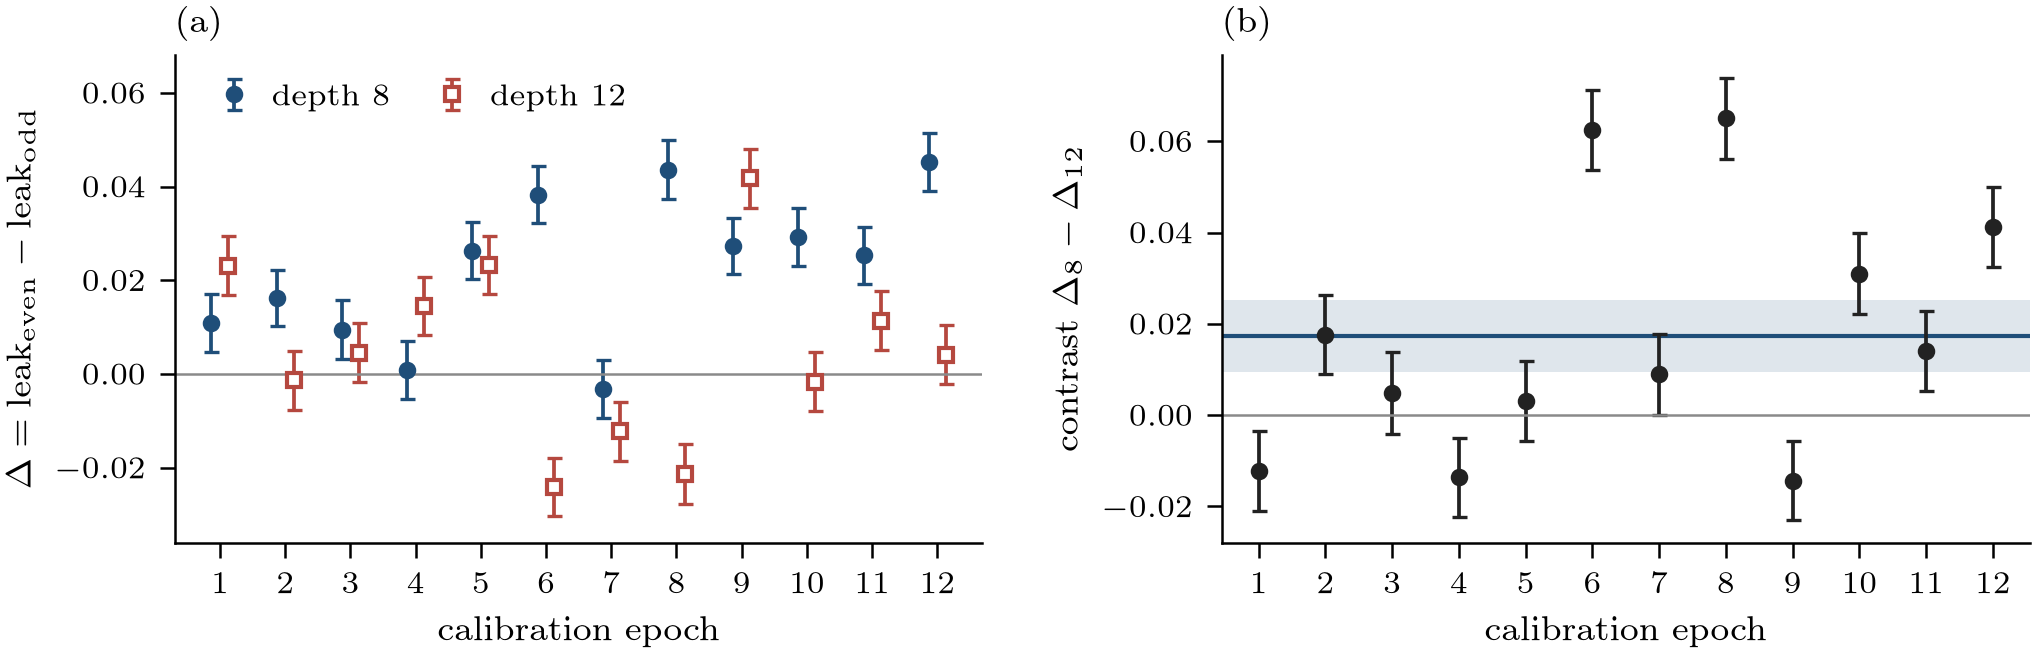
\includegraphics[width=0.98\linewidth]{figures/garnet_depth_contrast_twelve_epochs}
\caption{Twelve-epoch depth-ordering confirmation on Garnet. (a) Even-minus-odd leakage difference at depths 8 and 12 in each calibration epoch (12,288 shots per arm). (b) The preregistered contrast $\Delta_{8}-\Delta_{12}$ per epoch; the line and band are the random-effects mean and its standard error. Error bars are shot-noise standard errors and do not include the between-epoch spread.}
\label{fig:epochs}
\end{figure*}

The between-epoch $\tau$ is larger than the 0.0150 assumed when the sample size was
chosen, so the campaign had less power than the planned 0.92; the rejection
stands on the preregistered test as run, and the lower bound is close to zero.
The result is a statement about the mean over epochs: single epochs differ by
far more than their shot noise (per-epoch shot-noise standard error of the
contrast about 0.0088), and in three of twelve the sign is reversed.

\textbf{Secondary (preregistered).} Random-effects summaries of the asymmetry at
each depth separately: +0.0225 at depth 8 (standard error 0.0046, one-sided p
= 0.00024, \(\tau = 0.0146\)) and +0.0051 at depth 12 (standard error 0.0056, \(p = 0.19\), \(\tau = 0.0183\)). The six design epochs, which are not part of the endpoint,
had contrasts $-$0.0159, +0.0010, +0.0127, +0.0466, +0.0361 and +0.0202. The
four readout states of every epoch are committed with the counts and are not
used in the endpoint.

\begin{table*}[tb]
\centering
\footnotesize
\begin{tabular}{lllllll}
\toprule
epoch & date & calibration set & jobs (main, readout) & $\Delta_{8}$ & $\Delta_{12}$ & contrast \\
\midrule
1 & 2026-09-23 & \texttt{ad7e2bf0\ldots{}} & \texttt{01a0cfbc-c583\ldots{}}, \texttt{01a0cfbc-c711\ldots{}} & $+0.0109$ & $+0.0231$ & $-0.0122$ \\
2 & 2026-09-24 & \texttt{7c39177a\ldots{}} & \texttt{01a0d203-4e04\ldots{}}, \texttt{01a0d203-4fd7\ldots{}} & $+0.0162$ & $-0.0014$ & $+0.0176$ \\
3 & 2026-09-25 & \texttt{af33e1ea\ldots{}} & \texttt{01a0d916-2e1a\ldots{}}, \texttt{01a0d916-2f53\ldots{}} & $+0.0094$ & $+0.0046$ & $+0.0049$ \\
4 & 2026-09-26 & \texttt{d10715c4\ldots{}} & \texttt{01a0dec6-b2b3\ldots{}}, \texttt{01a0dec6-b3f0\ldots{}} & $+0.0008$ & $+0.0145$ & $-0.0137$ \\
5 & 2026-09-27 & \texttt{e1084b22\ldots{}} & \texttt{01a0e410-5e40\ldots{}}, \texttt{01a0e410-5f79\ldots{}} & $+0.0263$ & $+0.0233$ & $+0.0030$ \\
6 & 2026-09-29 & \texttt{a1a74f13\ldots{}} & \texttt{01a0ef34-e362\ldots{}}, \texttt{01a0ef34-e611\ldots{}} & $+0.0382$ & $-0.0242$ & $+0.0624$ \\
7 & 2026-10-01 & \texttt{36cf327c\ldots{}} & \texttt{01a0f933-9f69\ldots{}}, \texttt{01a0f933-a1de\ldots{}} & $-0.0033$ & $-0.0122$ & $+0.0090$ \\
8 & 2026-10-02 & \texttt{a4b99350\ldots{}} & \texttt{01a0fbf5-baa8\ldots{}}, \texttt{01a0fbf5-bc08\ldots{}} & $+0.0436$ & $-0.0214$ & $+0.0650$ \\
9 & 2026-10-03 & \texttt{0660d260\ldots{}} & \texttt{01a101dc-eada\ldots{}}, \texttt{01a101dc-ec11\ldots{}} & $+0.0273$ & $+0.0417$ & $-0.0144$ \\
10 & 2026-10-04 & \texttt{e431ada3\ldots{}} & \texttt{01a10729-ba87\ldots{}}, \texttt{01a10729-bd8d\ldots{}} & $+0.0293$ & $-0.0017$ & $+0.0310$ \\
11 & 2026-10-05 & \texttt{ff6836ae\ldots{}} & \texttt{01a10da8-ca46\ldots{}}, \texttt{01a10da8-cbf2\ldots{}} & $+0.0253$ & $+0.0113$ & $+0.0140$ \\
12 & 2026-10-06 & \texttt{6dd7fae6\ldots{}} & \texttt{01a11091-86f0\ldots{}}, \texttt{01a11091-890d\ldots{}} & $+0.0452$ & $+0.0041$ & $+0.0412$ \\
\bottomrule
\end{tabular}
\caption{Twelve-epoch depth-ordering confirmation. $\Delta$ is the even-minus-odd leakage difference at the given depth, pooled over the twelve repetitions of the epoch; the contrast is $\Delta_{8}-\Delta_{12}$. Calibration-set and provider job identifiers are abbreviated; the full identifiers are in the committed analysis artefact and submission journals.}
\label{tab:epochs}
\end{table*}

\textbf{Boundary.} A statement about device noise on IQM Garnet, this layout, these
two depths, this circuit family and this access period. Noiseless parity
leakage of these circuits is exactly zero, so nothing here is a statement
about coherent dynamics. No causal mechanism, no transfer to another backend,
no advantage claim.

\hypertarget{sec:8}{%
\section{Outlook: other devices and processor classes}\label{sec:8}}

Everything reported here and in our earlier work was measured on two families
of superconducting processors: heavy-hex IBM Heron r2 and square-lattice IQM
Garnet. The pooled even-over-odd sign of the parity-sector leakage asymmetry
is common to both; its depth dependence is not, and on Garnet it moves between
calibration epochs by more than the shot noise. Two devices cannot tell
whether these are properties of superconducting hardware in general, of
particular two-qubit-gate implementations, or of these two machines.

The measurement is small enough to be repeated on any current gate-model
processor: four qubits, number-conserving XY-Trotter circuits of depth 4 to
12, two initial states, and a few thousand shots per arm. Because the
noiseless parity leakage of these circuits is exactly zero, the observable is
a noise diagnostic that needs no classical reference beyond the counts
themselves. Processor classes whose dominant error channels, connectivity and
recalibration cadence differ from those of transmon devices --- trapped ions,
neutral atoms, spin qubits, and superconducting architectures with other
couplers or lattices --- are the informative comparison. We make no prediction
for them: an asymmetry of the same sign, of the opposite sign, or a bounded
null on another class would each constrain the explanation.

The protocol is published so that it can be run without us: the
preregistration texts, circuit builders, admission checks, submission journals
and frozen analysis scripts are in the public repository (Sec.~\ref{sec:9}). The one
design lesson we would carry over is the unit of analysis: on Garnet the
calibration epoch, not the shot, is the independent observation, and the
equivalent recalibration event of another platform should be identified before
the sample size is fixed. The confirmatory design used here costs twelve
epochs of 57,344 shots. We welcome replications by device operators and
independent groups, and would run the same preregistered protocol on other
hardware where access is available.

\hypertarget{sec:9}{%
\section{Reproducibility}\label{sec:9}}

Everything needed to reproduce all five campaigns is committed to the public
repository (github.com/anulum/scpn-quantum-control):

\begin{itemize}
\item
  preregistrations with frozen decision rules (and the amendment history);
\item
  live calibration snapshot with calibration-set identifier;
\item
  exact circuit payloads (QPY) and circuit-label manifests;
\item
  submission records with raw IQM job identifiers (publishable; the access
  token is never committed);
\item
  raw measurement counts for every reported hardware circuit;
\item
  for the twelve-epoch campaign, the per-epoch submission journals with the
  digest of every circuit payload written before the provider call, and the
  admission check each epoch passed before it was submitted;
\item
  frozen analysis scripts (fixed bootstrap seeds) whose committed artefacts
  contain every number quoted here;
\item
  the harness modules with 100\,\% test coverage, hermetic against synthetic
  lattices.
\end{itemize}

\hypertarget{sec:10}{%
\section{Claim boundaries}\label{sec:10}}

No quantum-advantage claim (all circuits are classically simulable at these
sizes --- that is what makes the exact references possible). No
coherence-protection claim. No coherent-dynamics claim for the parity
asymmetry (noiseless leakage is exactly zero). No layout-transfer claim
(the frozen rule failed). No extrapolation beyond the sampled device,
calibration windows, chain lengths, depths, and schedules. The core results
are statements about IQM Garnet on 2026-07-21 under calibration set
\texttt{246a4930-54e3-4cd9-a2d1-fcc0919675f5}; the per-size study is separately
bounded to its
2026-07-26 window under calibration set
\texttt{c2097be4-1e23-49bc-adaa-8e8c01df6223}. The window-variability and
depth-ordering results are statements about the pinned layout
{[}2, 7, 12, 13{]} over the windows and calibration epochs listed in Secs.~\ref{sec:6} and~\ref{sec:7}; a distinct calibration set marks an operational epoch and does not
prove physical independence, and the depth ordering is established for the
mean over twelve epochs, not for an individual epoch.

\begin{acknowledgments}
Quantum-hardware access was provided by \textbf{IQM} through the \textbf{IQM Resonance}
platform under an extended-access research grant. We thank the IQM support
team for the vetting and provisioning of that access.
\end{acknowledgments}

\renewcommand{\bibfont}{\footnotesize}
% Reference list as produced by BibTeX with apsrev4-2; kept inline because
% bibliography databases are not tracked under paper/.
%apsrev4-2.bst 2019-01-14 (MD) hand-edited version of apsrev4-1.bst
%Control: key (0)
%Control: author (72) initials jnrlst
%Control: editor formatted (1) identically to author
%Control: production of article title (-1) disabled
%Control: page (0) single
%Control: year (1) truncated
%Control: production of eprint (0) enabled
\begin{thebibliography}{14}%
\makeatletter
\providecommand \@ifxundefined [1]{%
 \@ifx{#1\undefined}
}%
\providecommand \@ifnum [1]{%
 \ifnum #1\expandafter \@firstoftwo
 \else \expandafter \@secondoftwo
 \fi
}%
\providecommand \@ifx [1]{%
 \ifx #1\expandafter \@firstoftwo
 \else \expandafter \@secondoftwo
 \fi
}%
\providecommand \natexlab [1]{#1}%
\providecommand \enquote  [1]{``#1''}%
\providecommand \bibnamefont  [1]{#1}%
\providecommand \bibfnamefont [1]{#1}%
\providecommand \citenamefont [1]{#1}%
\providecommand \href@noop [0]{\@secondoftwo}%
\providecommand \href [0]{\begingroup \@sanitize@url \@href}%
\providecommand \@href[1]{\@@startlink{#1}\@@href}%
\providecommand \@@href[1]{\endgroup#1\@@endlink}%
\providecommand \@sanitize@url [0]{\catcode `\\12\catcode `\$12\catcode
  `\&12\catcode `\#12\catcode `\^12\catcode `\_12\catcode `\%12\relax}%
\providecommand \@@startlink[1]{}%
\providecommand \@@endlink[0]{}%
\providecommand \url  [0]{\begingroup\@sanitize@url \@url }%
\providecommand \@url [1]{\endgroup\@href {#1}{\urlprefix }}%
\providecommand \urlprefix  [0]{URL }%
\providecommand \Eprint [0]{\href }%
\providecommand \doibase [0]{https://doi.org/}%
\providecommand \selectlanguage [0]{\@gobble}%
\providecommand \bibinfo  [0]{\@secondoftwo}%
\providecommand \bibfield  [0]{\@secondoftwo}%
\providecommand \translation [1]{[#1]}%
\providecommand \BibitemOpen [0]{}%
\providecommand \bibitemStop [0]{}%
\providecommand \bibitemNoStop [0]{.\EOS\space}%
\providecommand \EOS [0]{\spacefactor3000\relax}%
\providecommand \BibitemShut  [1]{\csname bibitem#1\endcsname}%
\let\auto@bib@innerbib\@empty
%</preamble>
\bibitem [{\citenamefont {Kuramoto}(1975)}]{Kuramoto1975}%
  \BibitemOpen
  \bibfield  {author} {\bibinfo {author} {\bibfnamefont {Y.}~\bibnamefont
  {Kuramoto}},\ }in\ \href@noop {} {\emph {\bibinfo {booktitle} {International
  Symposium on Mathematical Problems in Theoretical Physics}}}\ (\bibinfo
  {publisher} {Springer},\ \bibinfo {year} {1975})\ pp.\ \bibinfo {pages}
  {420--422}\BibitemShut {NoStop}%
\bibitem [{\citenamefont {Acebr{\'o}n}\ \emph {et~al.}(2005)\citenamefont
  {Acebr{\'o}n}, \citenamefont {Bonilla}, \citenamefont {{P{\'e}rez Vicente}},
  \citenamefont {Ritort},\ and\ \citenamefont {Spigler}}]{Acebron2005}%
  \BibitemOpen
  \bibfield  {author} {\bibinfo {author} {\bibfnamefont {J.~A.}\ \bibnamefont
  {Acebr{\'o}n}}, \bibinfo {author} {\bibfnamefont {L.~L.}\ \bibnamefont
  {Bonilla}}, \bibinfo {author} {\bibfnamefont {C.~J.}\ \bibnamefont
  {{P{\'e}rez Vicente}}}, \bibinfo {author} {\bibfnamefont {F.}~\bibnamefont
  {Ritort}},\ and\ \bibinfo {author} {\bibfnamefont {R.}~\bibnamefont
  {Spigler}},\ }\href {https://doi.org/10.1103/RevModPhys.77.137} {\bibfield
  {journal} {\bibinfo  {journal} {Reviews of Modern Physics}\ }\textbf
  {\bibinfo {volume} {77}},\ \bibinfo {pages} {137} (\bibinfo {year}
  {2005})}\BibitemShut {NoStop}%
\bibitem [{\citenamefont
  {{\v{S}}otek}(2026{\natexlab{a}})}]{SotekSoftware2026}%
  \BibitemOpen
  \bibfield  {author} {\bibinfo {author} {\bibfnamefont {M.}~\bibnamefont
  {{\v{S}}otek}},\ }\href {https://doi.org/10.5281/zenodo.18821929} {\bibinfo
  {title} {scpn-quantum-control: Quantum-native {SCPN} phase dynamics and
  control}} (\bibinfo {year} {2026}{\natexlab{a}})\BibitemShut {NoStop}%
\bibitem [{\citenamefont {{\v{S}}otek}(2026{\natexlab{b}})}]{SotekDLA2026}%
  \BibitemOpen
  \bibfield  {author} {\bibinfo {author} {\bibfnamefont {M.}~\bibnamefont
  {{\v{S}}otek}},\ }\href {https://doi.org/10.5281/zenodo.20382000} {\bibinfo
  {title} {Backend-sensitive hardware observation of parity-sector and
  excitation-number correlated decoherence asymmetry in the {XY}
  {H}amiltonian}} (\bibinfo {year} {2026}{\natexlab{b}})\BibitemShut {NoStop}%
\bibitem [{\citenamefont {Abdurakhimov}\ \emph {et~al.}(2024)\citenamefont
  {Abdurakhimov} \emph {et~al.}}]{Abdurakhimov2024}%
  \BibitemOpen
  \bibfield  {author} {\bibinfo {author} {\bibfnamefont {L.}~\bibnamefont
  {Abdurakhimov}} \emph {et~al.},\ }\href@noop {} {\bibinfo {title} {Technology
  and performance benchmarks of {IQM}'s 20-qubit quantum computer}} (\bibinfo
  {year} {2024}),\ \Eprint {https://arxiv.org/abs/2408.12433} {arXiv:2408.12433
  [quant-ph]} \BibitemShut {NoStop}%
\bibitem [{\citenamefont {Javadi-Abhari}\ \emph {et~al.}(2024)\citenamefont
  {Javadi-Abhari}, \citenamefont {Treinish}, \citenamefont {Krsulich},
  \citenamefont {Wood}, \citenamefont {Lishman}, \citenamefont {Gacon},
  \citenamefont {Martiel}, \citenamefont {Nation}, \citenamefont {Bishop},
  \citenamefont {Cross}, \citenamefont {Johnson},\ and\ \citenamefont
  {Gambetta}}]{Qiskit2024}%
  \BibitemOpen
  \bibfield  {author} {\bibinfo {author} {\bibfnamefont {A.}~\bibnamefont
  {Javadi-Abhari}}, \bibinfo {author} {\bibfnamefont {M.}~\bibnamefont
  {Treinish}}, \bibinfo {author} {\bibfnamefont {K.}~\bibnamefont {Krsulich}},
  \bibinfo {author} {\bibfnamefont {C.~J.}\ \bibnamefont {Wood}}, \bibinfo
  {author} {\bibfnamefont {J.}~\bibnamefont {Lishman}}, \bibinfo {author}
  {\bibfnamefont {J.}~\bibnamefont {Gacon}}, \bibinfo {author} {\bibfnamefont
  {S.}~\bibnamefont {Martiel}}, \bibinfo {author} {\bibfnamefont {P.~D.}\
  \bibnamefont {Nation}}, \bibinfo {author} {\bibfnamefont {L.~S.}\
  \bibnamefont {Bishop}}, \bibinfo {author} {\bibfnamefont {A.~W.}\
  \bibnamefont {Cross}}, \bibinfo {author} {\bibfnamefont {B.~R.}\ \bibnamefont
  {Johnson}},\ and\ \bibinfo {author} {\bibfnamefont {J.~M.}\ \bibnamefont
  {Gambetta}},\ }\href {https://doi.org/10.48550/arXiv.2405.08810} {\bibinfo
  {title} {Quantum computing with {Qiskit}}} (\bibinfo {year} {2024}),\ \Eprint
  {https://arxiv.org/abs/2405.08810} {arXiv:2405.08810 [quant-ph]} \BibitemShut
  {NoStop}%
\bibitem [{\citenamefont {Holm}(1979)}]{Holm1979}%
  \BibitemOpen
  \bibfield  {author} {\bibinfo {author} {\bibfnamefont {S.}~\bibnamefont
  {Holm}},\ }\href@noop {} {\bibfield  {journal} {\bibinfo  {journal}
  {Scandinavian Journal of Statistics}\ }\textbf {\bibinfo {volume} {6}},\
  \bibinfo {pages} {65} (\bibinfo {year} {1979})}\BibitemShut {NoStop}%
\bibitem [{\citenamefont {Cochran}(1954)}]{Cochran1954}%
  \BibitemOpen
  \bibfield  {author} {\bibinfo {author} {\bibfnamefont {W.~G.}\ \bibnamefont
  {Cochran}},\ }\href {https://doi.org/10.2307/3001666} {\bibfield  {journal}
  {\bibinfo  {journal} {Biometrics}\ }\textbf {\bibinfo {volume} {10}},\
  \bibinfo {pages} {101} (\bibinfo {year} {1954})}\BibitemShut {NoStop}%
\bibitem [{\citenamefont {Clopper}\ and\ \citenamefont
  {Pearson}(1934)}]{ClopperPearson1934}%
  \BibitemOpen
  \bibfield  {author} {\bibinfo {author} {\bibfnamefont {C.~J.}\ \bibnamefont
  {Clopper}}\ and\ \bibinfo {author} {\bibfnamefont {E.~S.}\ \bibnamefont
  {Pearson}},\ }\href {https://doi.org/10.1093/biomet/26.4.404} {\bibfield
  {journal} {\bibinfo  {journal} {Biometrika}\ }\textbf {\bibinfo {volume}
  {26}},\ \bibinfo {pages} {404} (\bibinfo {year} {1934})}\BibitemShut
  {NoStop}%
\bibitem [{\citenamefont {DerSimonian}\ and\ \citenamefont
  {Laird}(1986)}]{DerSimonianLaird1986}%
  \BibitemOpen
  \bibfield  {author} {\bibinfo {author} {\bibfnamefont {R.}~\bibnamefont
  {DerSimonian}}\ and\ \bibinfo {author} {\bibfnamefont {N.}~\bibnamefont
  {Laird}},\ }\href {https://doi.org/10.1016/0197-2456(86)90046-2} {\bibfield
  {journal} {\bibinfo  {journal} {Controlled Clinical Trials}\ }\textbf
  {\bibinfo {volume} {7}},\ \bibinfo {pages} {177} (\bibinfo {year}
  {1986})}\BibitemShut {NoStop}%
\bibitem [{\citenamefont {Hartung}\ and\ \citenamefont
  {Knapp}(2001)}]{HartungKnapp2001}%
  \BibitemOpen
  \bibfield  {author} {\bibinfo {author} {\bibfnamefont {J.}~\bibnamefont
  {Hartung}}\ and\ \bibinfo {author} {\bibfnamefont {G.}~\bibnamefont
  {Knapp}},\ }\href {https://doi.org/10.1002/sim.1009} {\bibfield  {journal}
  {\bibinfo  {journal} {Statistics in Medicine}\ }\textbf {\bibinfo {volume}
  {20}},\ \bibinfo {pages} {3875} (\bibinfo {year} {2001})}\BibitemShut
  {NoStop}%
\bibitem [{\citenamefont {Sidik}\ and\ \citenamefont
  {Jonkman}(2002)}]{SidikJonkman2002}%
  \BibitemOpen
  \bibfield  {author} {\bibinfo {author} {\bibfnamefont {K.}~\bibnamefont
  {Sidik}}\ and\ \bibinfo {author} {\bibfnamefont {J.~N.}\ \bibnamefont
  {Jonkman}},\ }\href {https://doi.org/10.1002/sim.1262} {\bibfield  {journal}
  {\bibinfo  {journal} {Statistics in Medicine}\ }\textbf {\bibinfo {volume}
  {21}},\ \bibinfo {pages} {3153} (\bibinfo {year} {2002})}\BibitemShut
  {NoStop}%
\bibitem [{\citenamefont {Knapp}\ and\ \citenamefont
  {Hartung}(2003)}]{KnappHartung2003}%
  \BibitemOpen
  \bibfield  {author} {\bibinfo {author} {\bibfnamefont {G.}~\bibnamefont
  {Knapp}}\ and\ \bibinfo {author} {\bibfnamefont {J.}~\bibnamefont
  {Hartung}},\ }\href {https://doi.org/10.1002/sim.1482} {\bibfield  {journal}
  {\bibinfo  {journal} {Statistics in Medicine}\ }\textbf {\bibinfo {volume}
  {22}},\ \bibinfo {pages} {2693} (\bibinfo {year} {2003})}\BibitemShut
  {NoStop}%
\bibitem [{\citenamefont {R{\"o}ver}\ \emph {et~al.}(2015)\citenamefont
  {R{\"o}ver}, \citenamefont {Knapp},\ and\ \citenamefont
  {Friede}}]{Roever2015}%
  \BibitemOpen
  \bibfield  {author} {\bibinfo {author} {\bibfnamefont {C.}~\bibnamefont
  {R{\"o}ver}}, \bibinfo {author} {\bibfnamefont {G.}~\bibnamefont {Knapp}},\
  and\ \bibinfo {author} {\bibfnamefont {T.}~\bibnamefont {Friede}},\ }\href
  {https://doi.org/10.1186/s12874-015-0091-1} {\bibfield  {journal} {\bibinfo
  {journal} {BMC Medical Research Methodology}\ }\textbf {\bibinfo {volume}
  {15}},\ \bibinfo {pages} {99} (\bibinfo {year} {2015})}\BibitemShut {NoStop}%
\end{thebibliography}%

\end{document}
